\section{Methods and Materials}

\subsection{Design of the Solution}

The Parking Management System was designed to automate and optimize the process of managing parking space availability, vehicle registration, and receipt generation. The solution aims to reduce human error, enhance operational efficiency, and offer a user-friendly interface for parking attendants.

The system follows a modular design approach, dividing it into several core components. The primary components include the frontend user interface (UI), the backend API (business logic), and the database. The frontend is responsible for interacting with parking attendants, allowing them to register vehicle entries and exits as well as generate receipts. The backend API processes the vehicle data, calculates parking fees, and communicates with the database to store or retrieve information. The database, based on PostgreSQL, stores data related to vehicles, parking slots, and receipts.

The technical decisions made during the design of the system were driven by the need for cost-effectiveness, scalability, and real-time data handling. The system was built to be low-cost, so that smaller parking lots could adopt it without significant financial investments. Additionally, scalability was considered in the design, allowing the system to handle increased usage if deployed in larger parking facilities. Real-time data handling ensures that parking attendants have up-to-date information on vehicle entry, exit, and parking space availability, contributing to improved operational control.\cite{webbylab2024smartparking}

\subsection{Technical Decisions}

Several key technologies were chosen for the development of the system. React was selected for the frontend because of its flexibility and ability to manage dynamic content efficiently. React allows for the creation of an interactive user interface where parking attendants can easily register vehicles, view parking space availability, and generate receipts.

For the backend, Flask was chosen due to its lightweight nature, scalability, and excellent support for building REST APIs. Flask’s simplicity made it an ideal choice to handle requests from the frontend, manage the business logic, and communicate with the database.

PostgreSQL was chosen as the database management system due to its robustness, ability to handle complex queries, and strong data integrity features. It was used to store vehicle data (such as license plates and entry/exit times) and receipt information (such as total parking duration and fees).

The CI/CD pipeline was implemented using GitHub Actions, automating the testing, building, and deployment of the system. Docker was used to containerize the system, ensuring consistency across development, testing, and production environments. The use of Docker Compose allowed for easy orchestration of the frontend, backend, and database containers, simplifying the deployment process.

\subsection{User Flow}

The system’s user flow is designed to be intuitive and efficient. When parking attendants log into the system, they are presented with the main interface. The primary tasks they will perform include registering vehicle entries, recording exits, and generating receipts.

Upon vehicle entry, the attendant enters the vehicle’s license plate number into the system, which logs the entry time and updates the parking space availability in real time. When the vehicle exits, the attendant registers the exit, and the system calculates the total parking duration and generates a receipt. All vehicle and receipt data is stored in the PostgreSQL database, ensuring data consistency and reliability.

\subsection{System Analysis and Architecture Design}

The system follows a client-server architecture. The client-side is the web-based interface that interacts with the parking attendants, and the server-side consists of the backend API and database. The frontend sends requests to the backend via REST APIs, which processes the data and returns the necessary information. The backend API interacts with the PostgreSQL database to store and retrieve vehicle and receipt data.

\subsubsection{Diagrams}

To enhance the understanding of the system’s design and its components, several diagrams were created to visualize the system:

\paragraph{Business Model Canvas:}
The Business Model Canvas was used to map out the value proposition, customer segments, revenue streams, channels, and key activities of the Parking Management System. This diagram helped align the system’s objectives with the overall business goals.

\begin{figure}[ht]
    \centering
    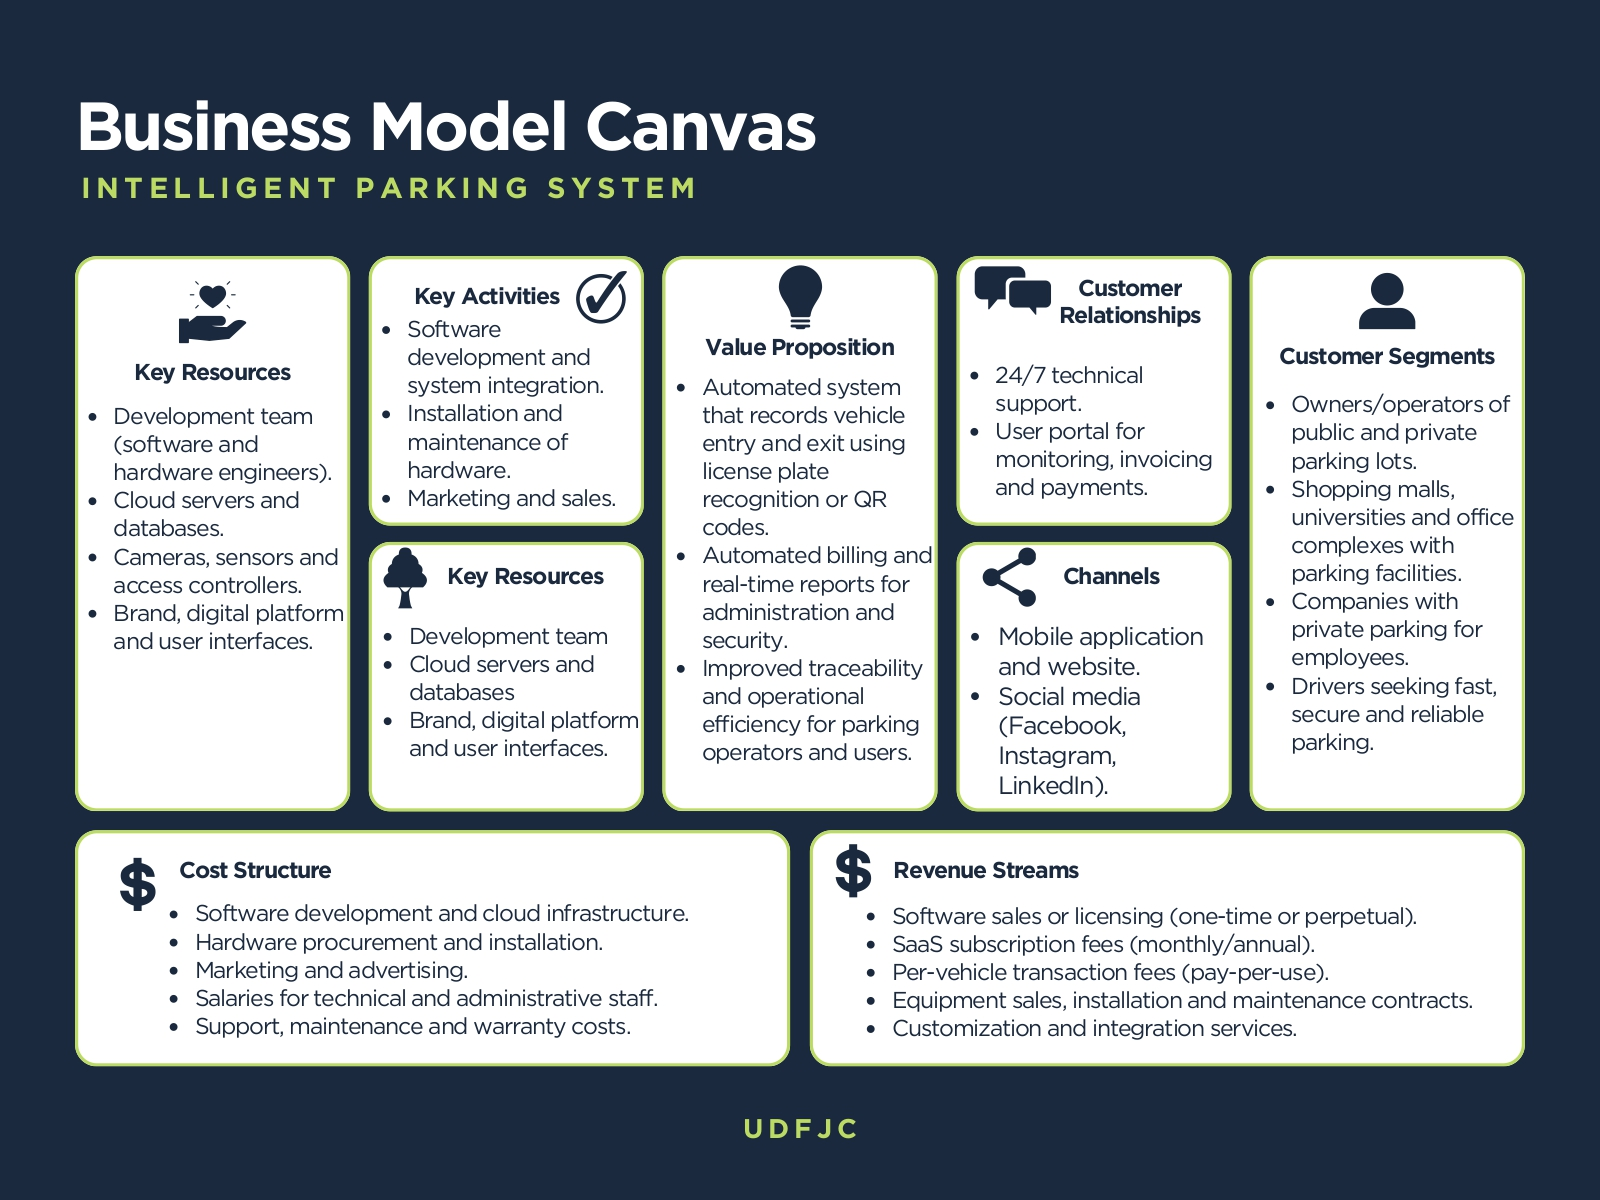
\includegraphics[width=0.8\linewidth]{methods/images/Business_Model_Canvas.jpg}
    \caption{Business Model Canvas for the Parking Management System}
\end{figure}

\paragraph{User Story Mapping:}
User Story Mapping was utilized to break down and prioritize the functionalities of the system from the perspective of parking attendants. It provided a visual representation of the system's features and their importance, helping to align development with user needs.

\begin{figure}[ht]
    \centering
    \includegraphics[width=0.8\linewidth]{methods/images/user_story_mapping.jpg}
    \caption{User Story Mapping for the Parking Management System}
\end{figure}

\paragraph{Class Diagram:}
The Class Diagram illustrates the object-oriented structure of the system. It shows the relationships between primary classes such as Vehicle, Receipt, and ParkingSlot. These classes represent the main entities in the system and their interactions.

\begin{figure}[ht]
    \centering
    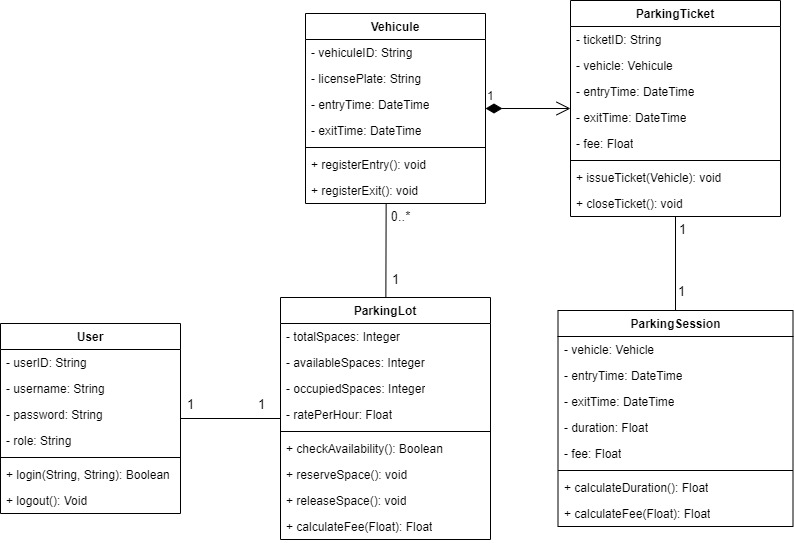
\includegraphics[width=0.8\linewidth]{methods/images/Class_Diagram_Parkinglot_System.jpg}
    \caption{Class Diagram for the Parking Management System}
\end{figure}

\paragraph{System Architecture Diagram:}
The System Architecture Diagram shows how the different components of the system interact with each other. It illustrates the flow of data between the frontend, backend, and database.

\begin{figure}[ht]
    \centering
    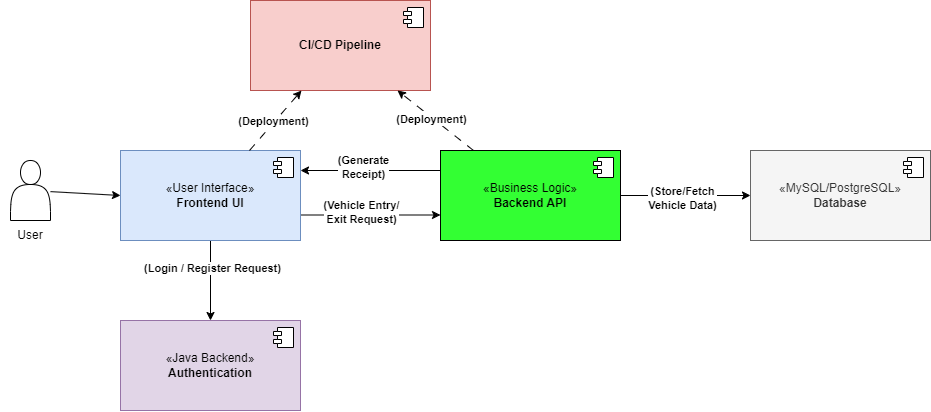
\includegraphics[width=0.8\linewidth]{methods/images/Parking_Management_System_Architecture.png}
    \caption{System Architecture Diagram for the Parking Management System}
\end{figure}

\paragraph{Deployment Diagram:}
The Deployment Diagram illustrates the physical deployment of the system across servers. It shows how the frontend, backend, and database are hosted and interact within the infrastructure, whether on-premises or in the cloud.

\begin{figure}[ht]
    \centering
    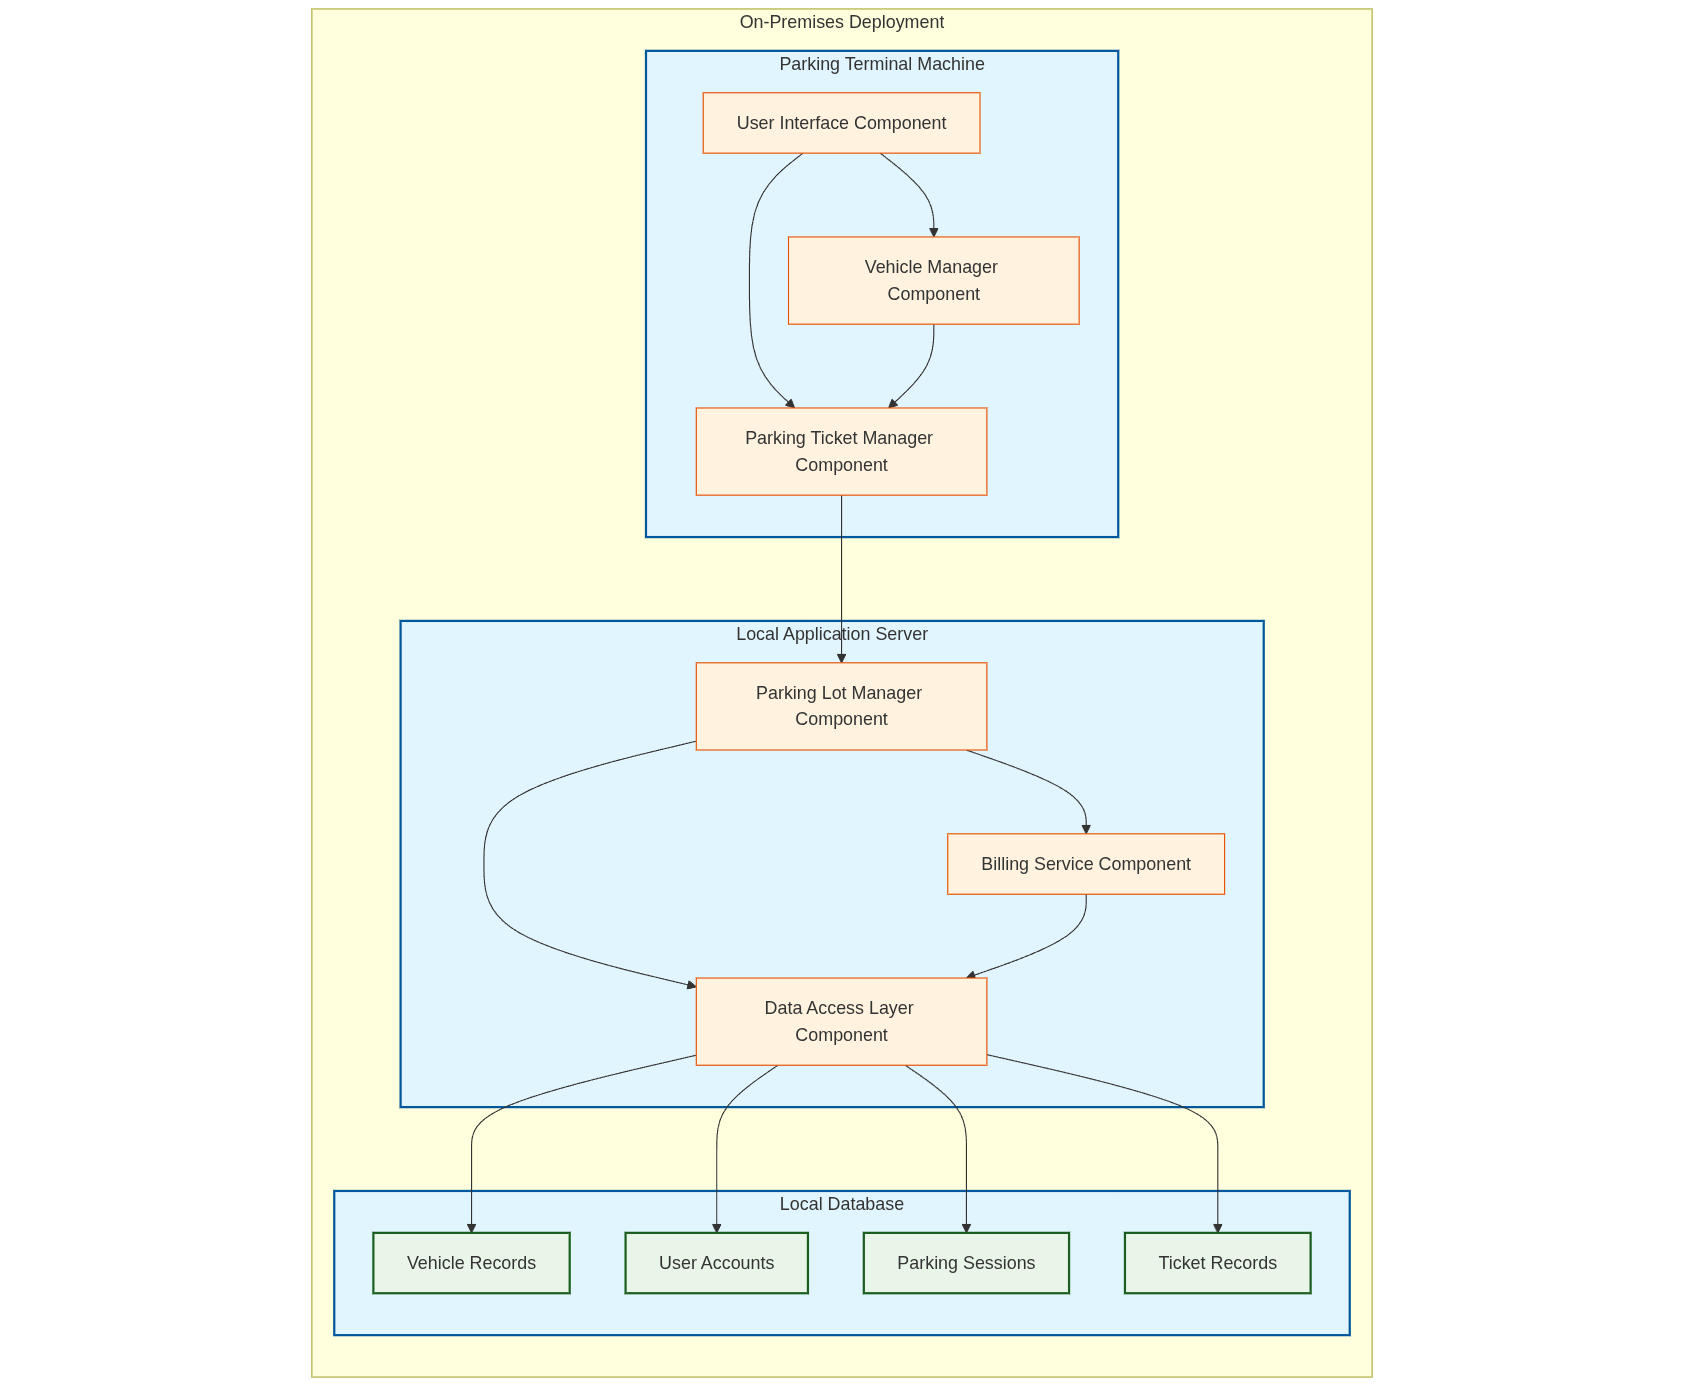
\includegraphics[width=0.8\linewidth]{methods/images/Deploy.png}
    \caption{Deployment Diagram for the Parking Management System}
\end{figure}

\paragraph{Business Process Diagram:}
The Business Process Diagram provides a visual representation of the steps involved in the parking management process, from vehicle entry to receipt generation. It helps visualize the flow of data and the interactions between the parking attendant and the system.

\begin{figure}[ht]
    \centering
    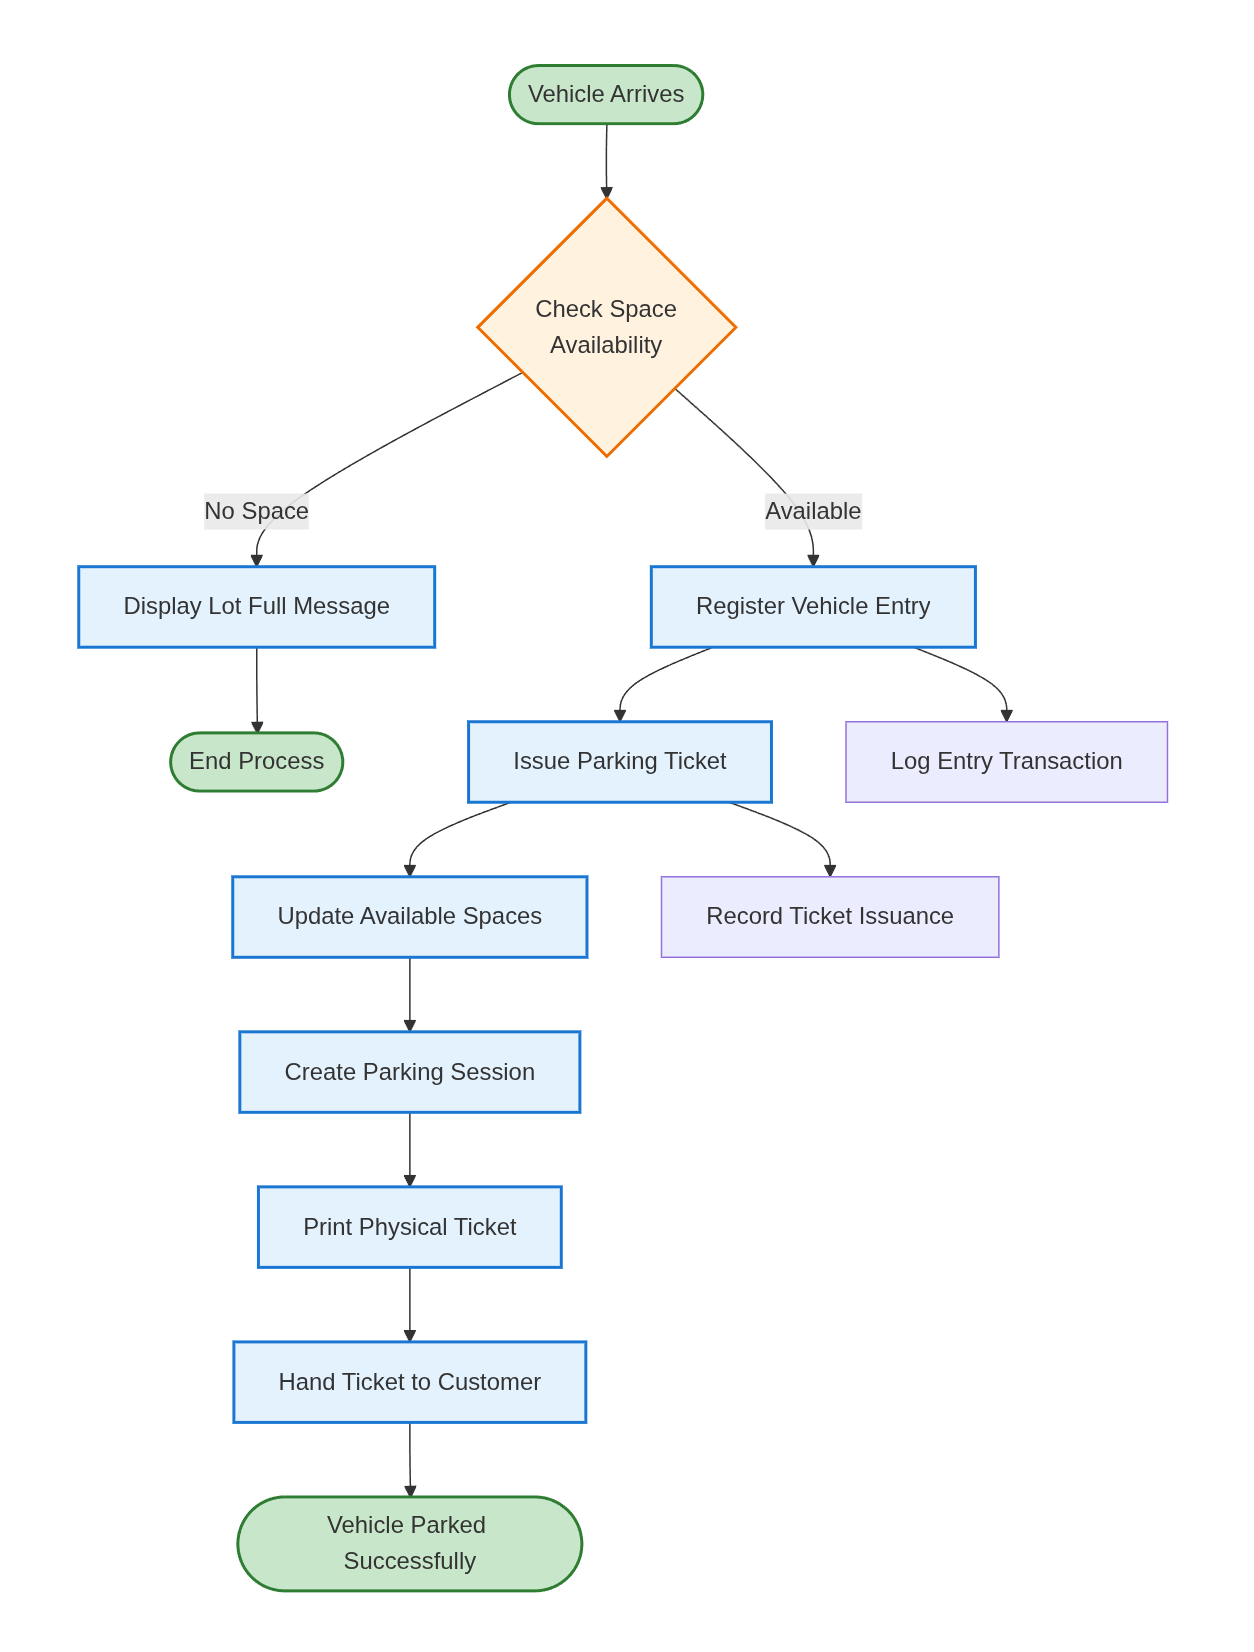
\includegraphics[width=0.8\linewidth]{methods/images/Bussiness.png}
    \caption{Business Process Diagram for the Parking Management System}
\end{figure}

\paragraph{Mockups:}
Three mockups were created to illustrate the key pages of the system’s frontend:
\begin{itemize}
    \item \textbf{Vehicle Registration Page}: Allows attendants to input vehicle details and register entries or exits.
    \item \textbf{Login/Register Page User}: Validates access credentials to manage and register vehicles entering and leaving the parking lot..
    \item \textbf{Dashboard for Parking Space Availability}: Shows real-time availability of parking spaces.
\end{itemize}

\begin{figure}[h]
    \centering
    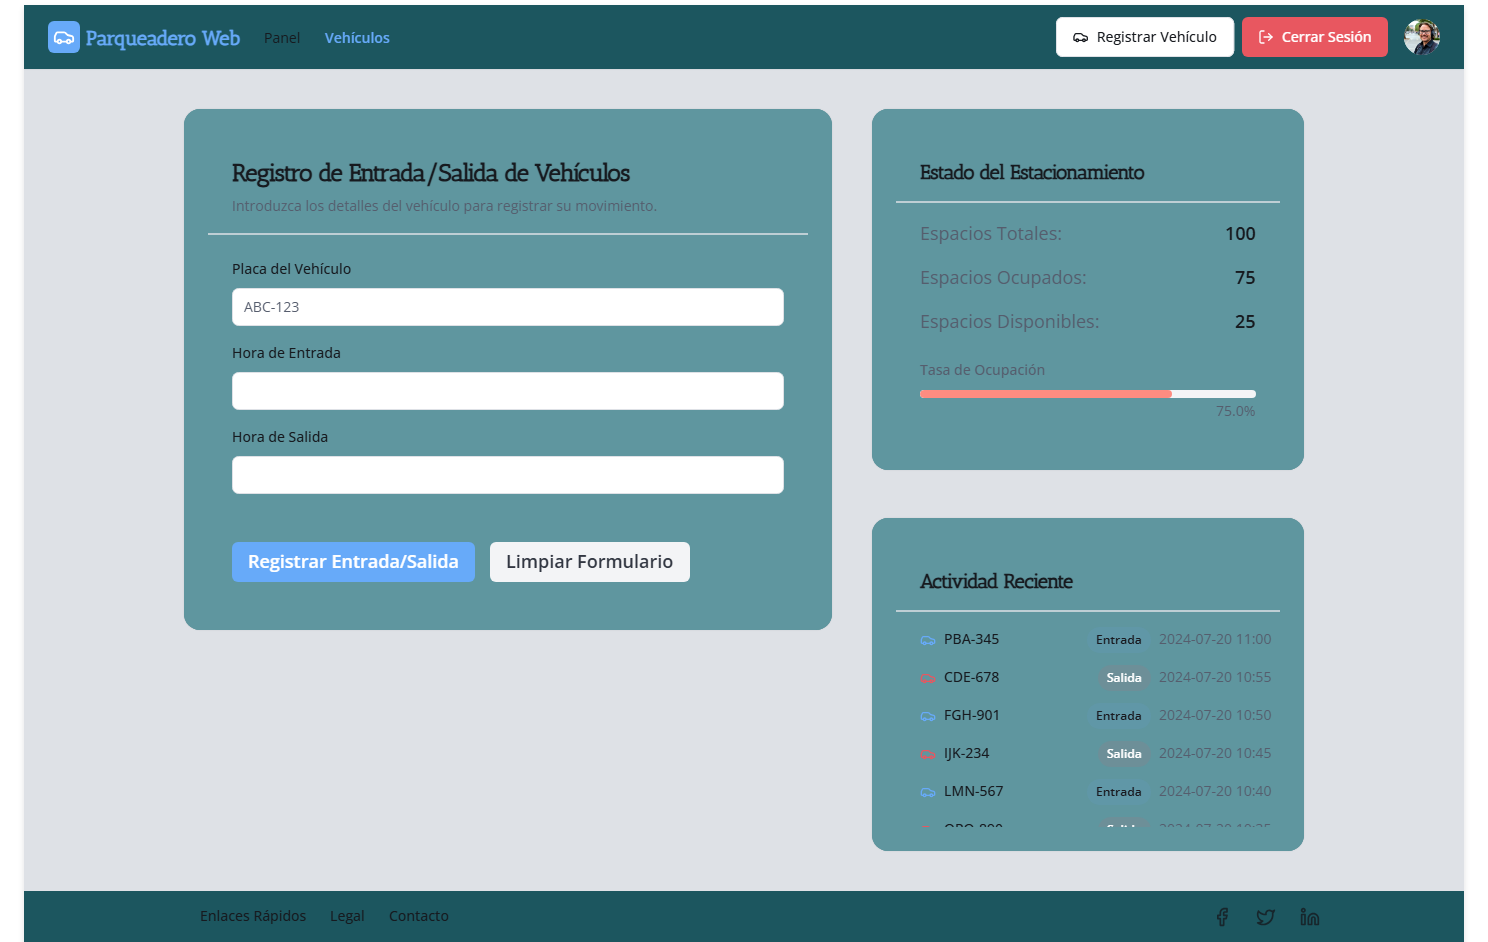
\includegraphics[width=0.8\linewidth]{methods/images/Mockup_Vehicle_Registration.png}
    \caption{Mockup of the Vehicle Registration Page}
\end{figure}

\begin{figure}[h]
    \centering
    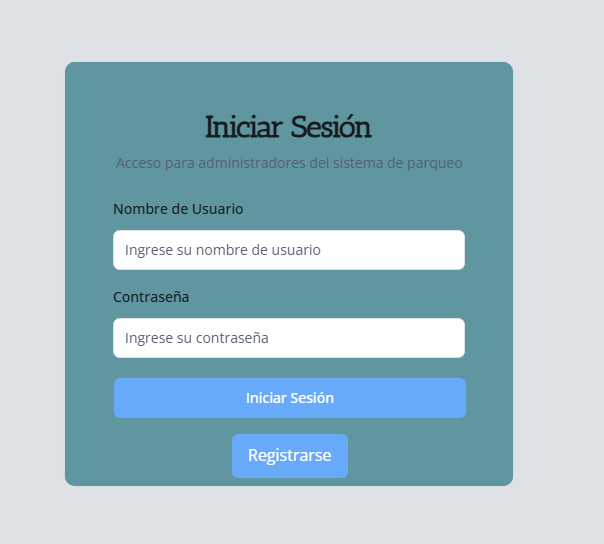
\includegraphics[width=0.8\linewidth]{methods/images/Mockup_Login.png}
    \caption{Mockup of the Login/Register Page User}
\end{figure}

\begin{figure}[h]
    \centering
    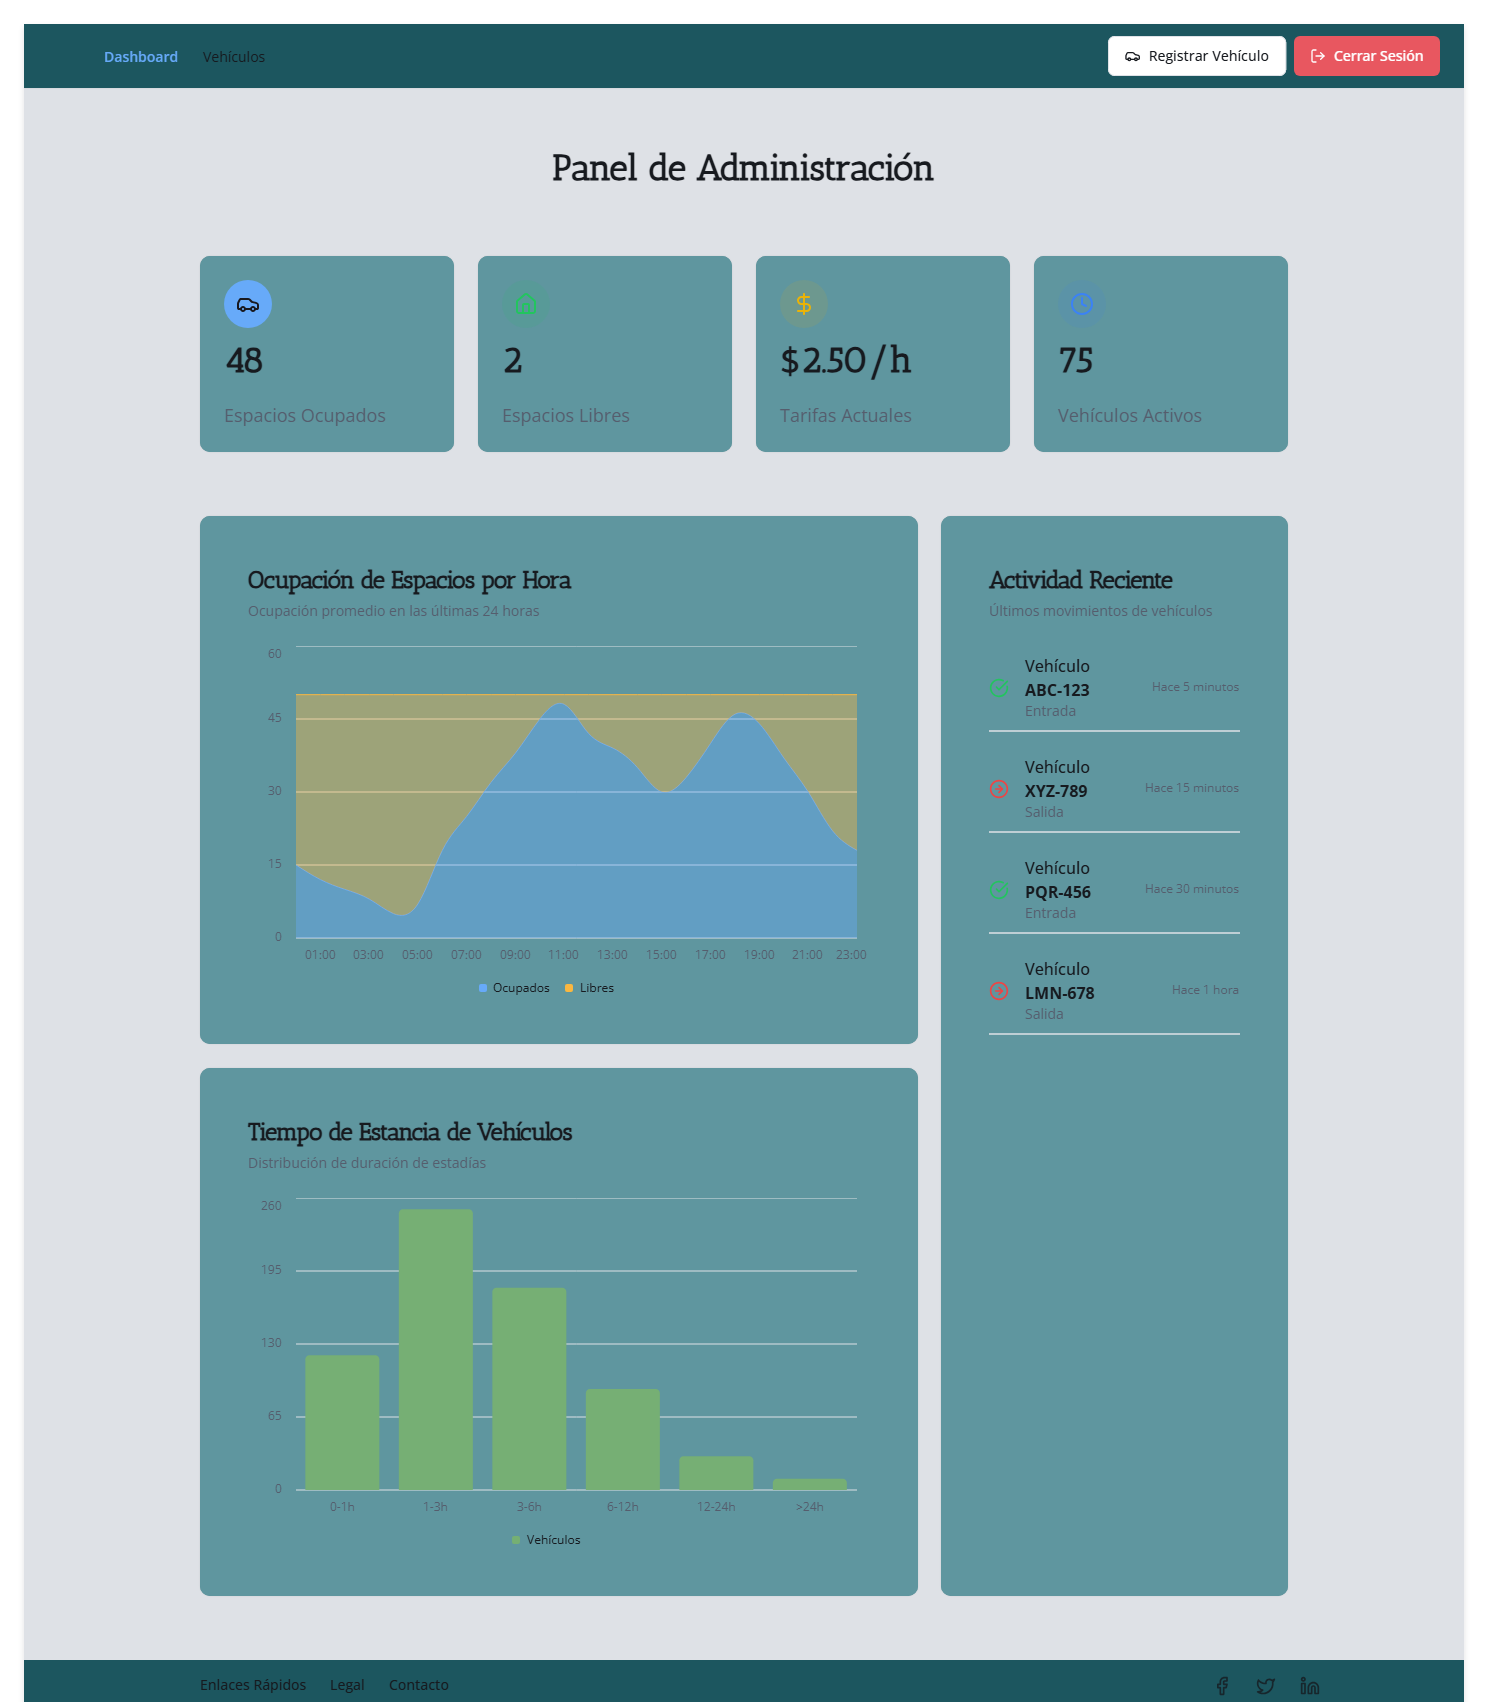
\includegraphics[width=0.8\linewidth]{methods/images/Mockup_Dashboard.png}
    \caption{Mockup of  Dashboard for Parking Space}
\end{figure}

\newpage

\subsection{CRC Cards}

\begin{tabular}{|p{0.5\columnwidth}|p{0.2\columnwidth}|}
    \hline
    \textbf{Class} & Vehicle\\
    \hline
    \textbf{Responsibilities} & \textbf{Collaborators}\\
    \hline
    \begin{tabular}{p{\columnwidth}}
         Known its own license plate\\
         Known its own car type\\
         Known its own brand\\
         Known its user owner\\
         \\
    \end{tabular}
     &
    \begin{tabular}{p{\columnwidth}}
        Slot \\
        User \\
        Register \\
    \end{tabular}  \\
    \hline
\end{tabular}\\\\

\begin{tabular}{|p{0.5\columnwidth}|p{0.2\columnwidth}|}
    \hline
    \textbf{Class} & User\\
    \hline
    \textbf{Responsibilities} & \textbf{Collaborators}\\
    \hline
    \begin{tabular}{p{8.5cm}}
        Known its own id \\
        Known its user type \\
        Manage associated cars \\
        Known its own brand \\
        Known its user owner \\
    \end{tabular}
     &
    \begin{tabular}{p{4.5cm}}
        Slot \\
        Vehicle \\
        Register \\
    \end{tabular}  \\
    \hline
\end{tabular}\\\\

\begin{tabular}{|p{0.5\columnwidth}|p{0.2\columnwidth}|}
    \hline
    \textbf{Class} & Fee\\
    \hline
    \textbf{Responsibilities} & \textbf{Collaborators}\\
    \hline
    \begin{tabular}{p{8.5cm}}
        Known prices per hour \\
        Known prices by vehicle type \\
        Known special fees by user \\
        Apply discounts by user type \\
    \end{tabular}
     &
    \begin{tabular}{p{4.5cm}}
        User \\
        Register \\
    \end{tabular}  \\
    \hline
\end{tabular}\\\\

\begin{tabular}{|p{0.5\columnwidth}|p{0.2\columnwidth}|}
    \hline
    \textbf{Class} & Register\\
    \hline
    \textbf{Responsibilities} & \textbf{Collaborators}\\
    \hline
    \begin{tabular}{p{8.5cm}}
        Register vehicule entry \\
        Register vehicule departure \\
        Calculate vehicule parking time \\
        Calculete cost \\
        Apply user discounts \\
        Generate ticket \\
    \end{tabular}
     &
    \begin{tabular}{p{4.5cm}}
        Vehicle \\
        User \\
        Fee \\
        slot \\
    \end{tabular}  \\
    \hline
\end{tabular}\\\\

\begin{tabular}{|p{0.5\columnwidth}|p{0.2\columnwidth}|}
    \hline
    \textbf{Class} & Slot\\
    \hline
    \textbf{Responsibilities} & \textbf{Collaborators}\\
    \hline
    \begin{tabular}{p{8.5cm}}
        Know its own id \\
        Know if it's free \\
        Know its own slot type \\
        Reserve \\
        Get empty \\
    \end{tabular}
     &
    \begin{tabular}{p{4.5cm}}
        Vehicle \\
        Register \\
        Area \\
    \end{tabular}  \\
    \hline
\end{tabular}\\\\

\begin{tabular}{|p{0.5\columnwidth}|p{0.2\columnwidth}|}
    \hline
    \textbf{Class} & Area\\
    \hline
    \textbf{Responsibilities} & \textbf{Collaborators}\\
    \hline
    \begin{tabular}{p{8.5cm}}
        Know its own id \\
        Know its own name \\
        Know its own capacity \\
        Know its own slots disponibility \\
    \end{tabular}
     &
    \begin{tabular}{p{4.5cm}}
        Slot \\
        Register \\
    \end{tabular}  \\
    \hline
\end{tabular}\\\\

\subsection{Conclusion of Methods and Materials}

The Parking Management System was designed with simplicity, scalability, and usability in mind. The system was divided into modular components to ensure that each aspect of the parking process — from vehicle registration to receipt generation — is streamlined and automated. By using modern technologies such as Flask, PostgreSQL, and Docker, the system ensures reliability, scalability, and ease of deployment. The diagrams and mockups provided help visualize the design, user flow, and architecture of the system.
